\documentclass{article}
\usepackage{tikz}
\usetikzlibrary{arrows.meta}

\begin{document}

\begin{figure}[h]
    \centering
    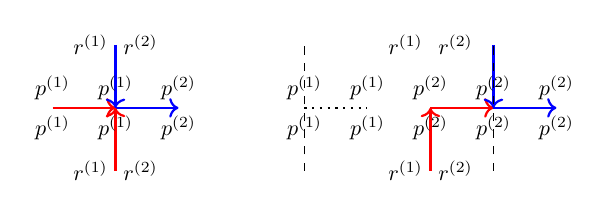
\begin{tikzpicture}[scale=0.8, every node/.style={scale=0.8}]
        
        % Left subfigure
        \draw[thick, ->, red] (-1,0) -- (0,0);
        \draw[thick, ->, blue] (0,0) -- (1,0);
        \draw[thick, ->, red] (0,-1) -- (0,0);
        \draw[thick, ->, blue] (0,1) -- (0,0);
        
        \node at (-1,0) [above] {$p^{(1)}$};
        \node at (-1,0) [below] {$p^{(1)}$};
        \node at (0,0) [above] {$p^{(1)}$};
        \node at (0,0) [below] {$p^{(1)}$};
        \node at (1,0) [above] {$p^{(2)}$};
        \node at (1,0) [below] {$p^{(2)}$};
        \node at (0,1) [left] {$r^{(1)}$};
        \node at (0,-1) [left] {$r^{(1)}$};
        \node at (0,1) [right] {$r^{(2)}$};
        \node at (0,-1) [right] {$r^{(2)}$};
        
        % Right subfigure
        \draw[dotted, thick] (3,0) -- (4,0);
        \draw[thick, ->, red] (5,0) -- (6,0);
        \draw[thick, ->, blue] (6,0) -- (7,0);
        \draw[thick, ->, red] (5,-1) -- (5,0);
        \draw[thick, ->, blue] (6,1) -- (6,0);
        
        \node at (3,0) [above] {$p^{(1)}$};
        \node at (3,0) [below] {$p^{(1)}$};
        \node at (4,0) [above] {$p^{(1)}$};
        \node at (4,0) [below] {$p^{(1)}$};
        \node at (5,0) [above] {$p^{(2)}$};
        \node at (5,0) [below] {$p^{(2)}$};
        \node at (6,0) [above] {$p^{(2)}$};
        \node at (6,0) [below] {$p^{(2)}$};
        \node at (7,0) [above] {$p^{(2)}$};
        \node at (7,0) [below] {$p^{(2)}$};
        \node at (5,1) [left] {$r^{(1)}$};
        \node at (5,-1) [left] {$r^{(1)}$};
        \node at (5,1) [right] {$r^{(2)}$};
        \node at (5,-1) [right] {$r^{(2)}$};
        
        % Dashed lines
        \draw[dashed] (3,-1) -- (3,1);
        \draw[dashed] (6,-1) -- (6,1);
        
    \end{tikzpicture}
    \caption{The left subfigure in each panel, with red arrows, represents a vertex in system 1, and the right subfigure, with blue arrows, represents a vertex in system 2; notice that each system is a uncolored, so here blue and red do not represent colors (in the sense of priority) associated to the arrows as in the main text of the paper. Black edges represent an absence of an arrow. For $i\in\{1,2\}$, in system $i$, the label of the horizontally incoming arrow is $p^{(i)}$, and that of the vertically incoming arrow is $r^{(i)}$. The outgoing labels are assigned as depicted.}
    \label{fig:example}
\end{figure}

\end{document}